\section{Probabilistic and Nondeterministic Systems}
\label{sec:background:probabilistic-stochastic}

Probabilistic and nondeterministic systems are those by which, for the same given input, different outcomes may result. The underlying models that power an \gls{iws} are treated as though they are nondeterministic; \cref{ch:background} introduces \glspl{iws} as essentially black-box behaviour that can change over time. As such, we adopt the nondeterministic behaviour that they present.

\begin{figure}[h!]
  \centering
  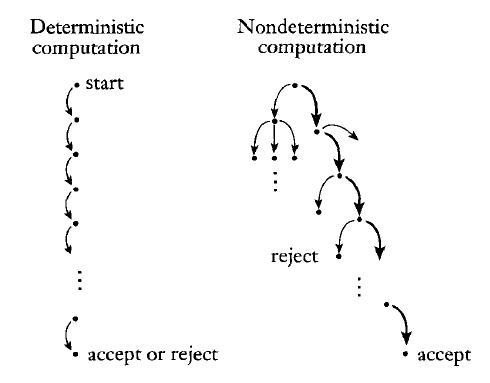
\includegraphics[width=0.6\linewidth]{nfa-compute}
  \caption[Deterministic versus nondeterministic systems]{A deterministic system (left) always returns the same result in the same amount of steps. A nondeterministic system does not guarantee the same outcome, even with the same input data. Source:~\citep{Finalyson:2018aa}.}
  \label{fig:background:probabilistic-stochastic:nfa-compute}
\end{figure}

\subsection{Interpreting the Uninterpretable}
\label{ssec:background:probabilistic-stochastic:model-interpretability}

As the rise of applied \gls{ai} increases, the need for engineering interpretability around models becomes paramount, chiefly from an external quality perspective that the \textit{reliability} of the system can be inspected by end-users. Model interpretability has been stressed since early machine learning research in the late 1980s and 1990s (such as \citet{Quinlan:1999ue} and \citet{Michie:1988te}), and although there has since been a significant body of work in the area \citep{Singh:2016wu,Baehrens:2010tj,Ribeiro:2016gg,Bussone:2015wm,Ross:2017vn,Lipton:2016if,Boz:2002uv,Johansson:2009uo,Augasta:2012wx,Fung:2005we,Dejaeger:2012up,VanAssche:2007wc,BenDavid:1995up,Feelders:2000ve,Lima:2009tm,Martens:2011uh,Pazzani:1997vp,Verbeke:2011vo}, it is evident that `accuracy' or model `confidence' is still used as a primary criterion for AI evaluation \citep{Huang:2005tc,Japkowicz:2011vy,Sokolova:2009vu}. Much research into \glsx{nn} or \glsx{svm} development stresses that `good' models are those with high accuracy. However, is accuracy enough to justify a model's quality?

To answer this, we revisit what it means for a model to be accurate. Accuracy is an indicator for estimating how well a model's algorithm will work with future or unforeseen data. It is quantified in the \gls{ai} testing stage, whereby the algorithm is tested against cases known by humans to have ground truth but such cases are unknown by the algorithm. In production, however, all cases are unknown by both the algorithm \textit{and} the humans behind it, and therefore a single value of quality is ``not reliable if the future dataset has a probability distribution significantly different from past data'' \citep{Freitas:2014ic}, a problem commonly referred to as the \textit{datashift} problem \citep{Sugiyama:2017ud}. Analogously, \citet{Freitas:2014ic} provides the following description of the problem:

\begin{quote}
\itshape
The military trained [a \gls{nn}] to classify images of tanks into enemy and friendly tanks. However, when the [\gls{nn}] was deployed in the field (corresponding to ``future data''), it had a poor accuracy rate. Later, users noted that all photos of friendly (enemy) tanks were taken on a sunny (overcast) day. I.e., the [\gls{nn}] learned to discriminate between the colors of the sky in sunny vs. overcast days! \textbf{If the [\gls{nn}] had output a comprehensible model (explaining that it was discriminating between colors at the top of the images), such a trivial mistake would immediately be noted.}
\upshape
\citep{Freitas:2014ic}
\end{quote}

So, why must we interpret models? While the formal definition of what it means to be \textit{interpretable} is still somewhat disparate (though some suggestions have been proposed \citep{Lipton:2016if}), what is known is (i) there exists a critical trade-off between accuracy and interpretability \citep{Freitas:2004vv,Jin:2006uf,Kaufman:1999vg,Grunwald:2007vg,Domingos:1998ug,Zahalka:2011ux}, and (ii) a single quantifiable value cannot satisfy the subjective needs of end-users \citep{Freitas:2014ic}. As ever-growing domains \gls{ml} become widespread\footnote{In areas such as medicine \citep{Bellazzi:2008tv,Lavrac:1999tf,Pazzani:2001tw,Richards:2001vw,Zupan:2000tp,VanAssche:2007wc,Johansson:2009uo,Elazmeh:2007tp,Wong:2006ve,Jaspers:2011hy,Bussone:2015wm}, bioinformatics \citep{Freitas:2010vk,Szafron:2004uf,Karwath:2002tv,Doderer:2006vt,Jiang:2005ua}, finance \citep{Baehrens:2010tj,Huysmans:2011gq,Dhar:2000vo} and customer analytics \citep{Verbeke:2011vo,Lima:2009tm}.}, these applications engage end-users for real-world goals, unlike the aims in early \gls{ml} research where the aim was to get \gls{ai} working in the first place. In safety-critical systems where \gls{ai} provide informativeness to humans to make the final call (see \citep{Caruana:2015jk,Kim:2015vo,Huysmans:2011gq}), there is often a mismatch between the formal objectives of the model (e.g., to minimise error) and complex real-world goals, where other considerations (such as the human factors and cognitive science behind explanations\footnote{\textit{Interpretations} and \textit{explanations} are often used interchangeably.}) are not realised: model optimisation is only worthwhile if they ``actually solve the original [human-centred] task of providing explanation'' \citep{Narayanan:2018ud} to end-users. \textbf{Therefore, when human-decision makers must be interpretable themselves \citep{Ridgeway:1998ud}, any \gls{ai} they depend on must also be interpretable.} 

Recently, discussion behind such a notion to provide legal implications of interpretability is topical. \citet{DoshiVelez:2017vm} discuss when explanations are not provided from a legal stance---for instance, those affected by algorithmic-based decisions have a `right to explanation' \citep{Goodman:2016wf,Wachter:2017hx} under the European Union's GDPR\footnoteurl{https://www.eugdpr.org}{13 August 2018}. But, explanations are not the only way to ensure \gls{ai} accountability: theoretical guarantees (mathematical proofs) or statistical evidence can also serve as guarantees \citep{DoshiVelez:2017vm}, however, in terms of explanations, what form they take and how they are proven correct are still open questions \citep{Lipton:2016if}.

\subsection{Explanation and Communication}
\label{ssec:background:probabilistic-stochastic:communication}

From a software engineering perspective, explanations and interpretability are, by definition, inherently communication issues: what lacks here is a consistent interface between the \gls{ai} system and the person using it. The ability to encode `common sense reasoning' \citep{McCarthy:1960:PCS:889202} into programs today has been achieved, but \textit{decoding} that information is what still remains problematic. At a high level, \citeauthor{Shannon:1963ti}'s theory of communication \citep{Shannon:1963ti} applies, just as others have done with similar issues in the software engineering realm \citep{Moody:2009vo,Wickham:2010hy} (albeit to the domain of visual notations). Humans map the world in higher-level concepts easily when compared to \gls{ai} systems: while we think of a tree first (not the photons of light or atoms that make up the tree), an algorithm simply sees pixels, and not the concrete object \citep{DoshiVelez:2017vm} and the \gls{ai} interprets the tree inversely to humans. Therefore, the interpretation or explanation is done inversely: humans do not explain the individual neurons fired to explain their predictions, and therefore the algorithmic transparent explanations of \gls{ai} algorithms (\textit{``which neurons were fired to make this \gls{ai} think this tree is a tree?''}) do not work here.

Therefore, to the user (as mapped using \citeauthor{Shannon:1963ti}'s theory), an AI pipeline (the communication \textit{channel}) begins with a real-world concept, $y$, that acts as an \textit{information source}. This information source is fed in as a \textit{message}, $x$, (as pixels) to an AI system (the \textit{transmitter}). The transmitter encodes the pixels to a prediction, $\hat{y}$, the \textit{signal} of the message. This signal is decoded by the \textit{receiver}, an explanation system, $e_{x}(x,\hat{y})$, that tailors the prediction with the given input data to the intended end user (the \textit{destination}) as an explanation,~$\tilde{y}$, another type of \textit{message}. Therefore, the user only sees the channel as an input/output pipeline of real-world objects, $y$, and explanations, $\tilde{y}$, tailored to \textit{them}, without needing to see the inner-mechanics of a prediction $\hat{y}$. We present this diagrammatically in \cref{fig:background:probabilistic-stochastic:theory-of-ai-communication}.

\begin{figure}[t!]
  \centering
  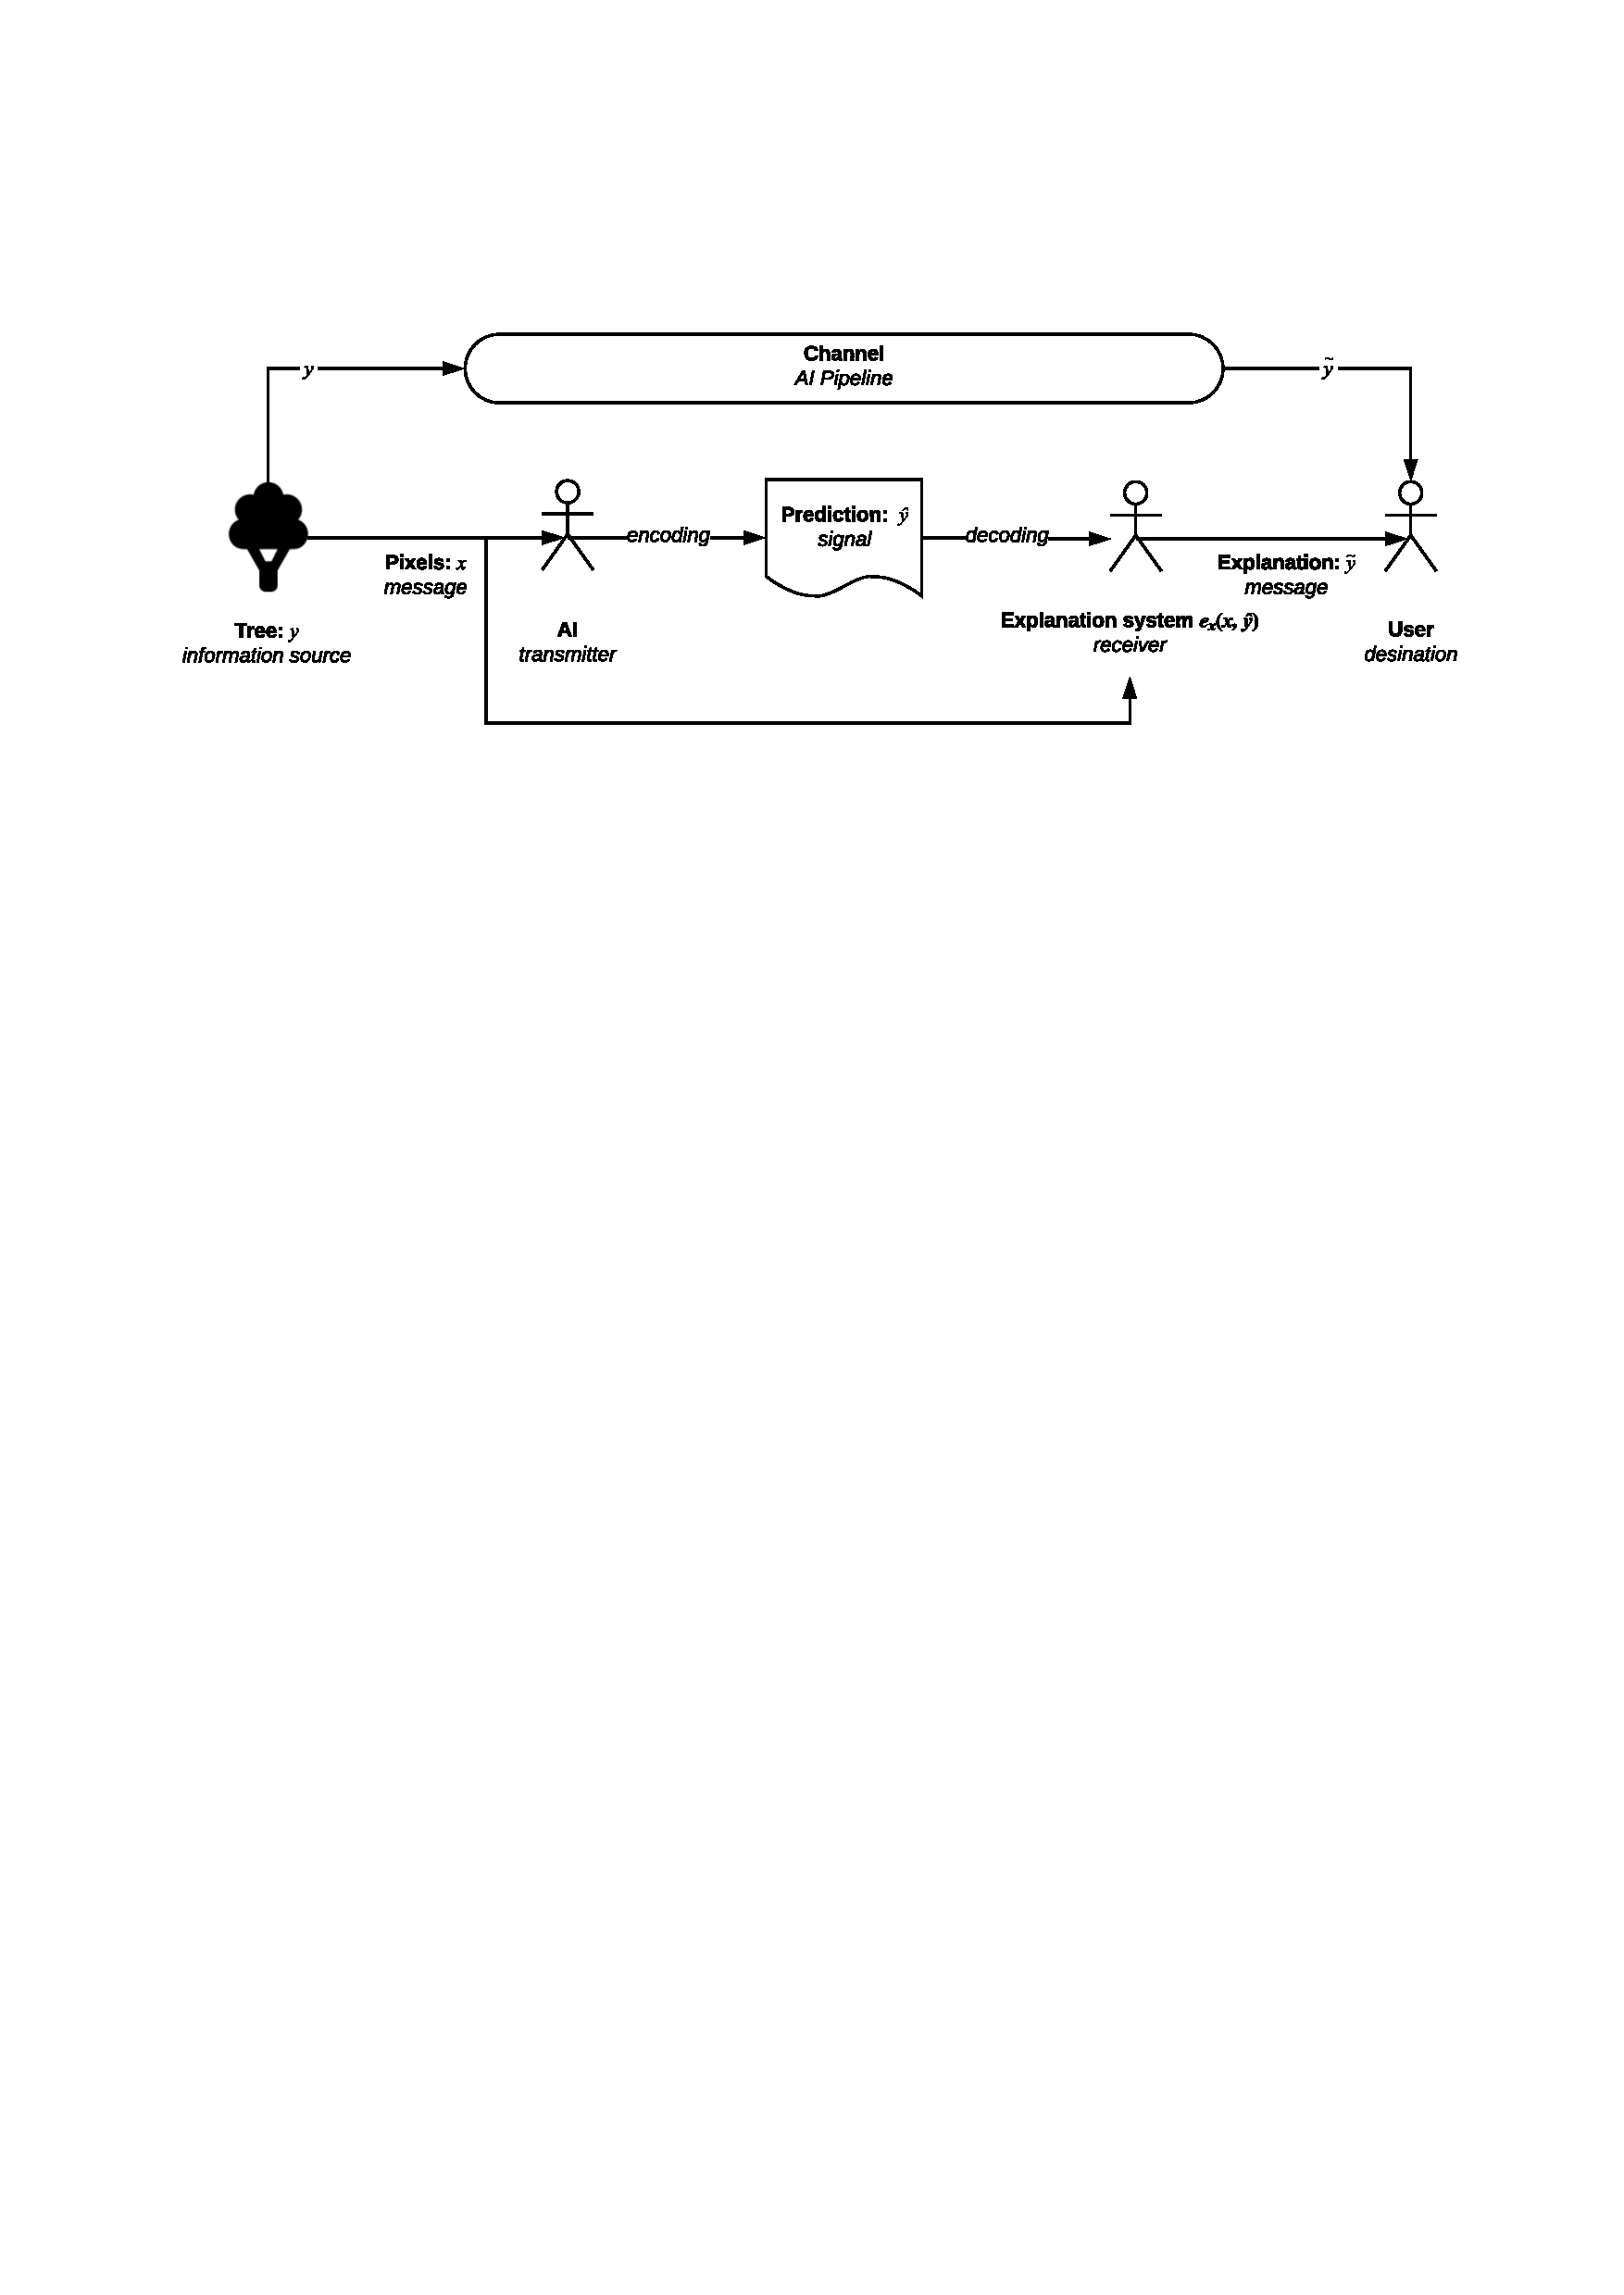
\includegraphics[width=\textwidth]{communication}
  \caption[Theory of AI communication]{Theory of AI communication from information source, $y$, to intended user as explanations, $\tilde{y}$.}
  \label{fig:background:probabilistic-stochastic:theory-of-ai-communication}
\end{figure}

\subsection{Mechanics of Model Interpretation}
\label{ssec:background:probabilistic-stochastic:mechanics}

How do we interpret models? Methods for developing interpretation models include: decision trees \citep{Breiman:1984tu,Hastie:2001wp,Craven:1995wg,Quinlan:1993vi,Rokach:2008wc}, decision tables \citep{Lima:2009tm,Baesens:2003we} and decision sets \citep{Lakkaraju:2016ka,Narayanan:2018ud}; input gradients, gradient vectors or sensitivity analysis \citep{Selvaraju:2017bk,Ribeiro:2016gg,Lei:2016wi,Ross:2017vn,Baehrens:2010tj}; exemplars \citep{Kim:2014ui,Frey:2007hs}; generalised additive models \citep{Caruana:2015jk}; classification (\textit{if-then}) rules \citep{Thrun:1996wh,Bramer:2007vg,Clark:1991vi,Otero:2013ul,Witten:2016ut} and falling rule lists \citep{Singh:2016wu}; nearest neighbours \citep{Martens:2011uh,Sen:1995uk,Suri:2007wl,Wettschereck:1997vw,Zhang:2008vfa} and Na\"{i}ve Bayes analysis \citep{Bellazzi:2008tv,Lavrac:1999tf,Kononenko:1993td,Zupan:2000tp,Michie:1994wi,Friedman:1997vs,Cheng:2001vw,Heckerman:2000uw}. 

Cross-domain studies have assessed the interpretability of these techniques against end-users, measuring response time, accuracy in model response and user confidence \citep{Huysmans:2011gq,Hayete:2005tn,Allahyari:2011ud,Subramanian:1992ue,Schwabacher:2001wc,Freitas:2010vk,Martens:2011uh,Verbeke:2011vo}, although it is generally agreed that decision rules and decision tables provide the most interpretation in non-linear models such as \glspl{svm} or \glspl{nn} \citep{Freitas:2010vk,Martens:2011uh,Verbeke:2011vo}. For an extensive survey of the benefits and fallbacks of these techniques, we refer to \citet{Freitas:2014ic}, \citet{DoshiVelez:2017vm} and \citet{DoshiVelez:2017wu}.

An important factor in model interpretation is to avoid over-reliance, and thus, one mechanism of model interpretation is to reduce explanations  altogether. For example, \citet{Bussone:2015wm} showed that, in clinical decision support systems, confidence values alone only results in a slight effect on trust and reliance of a system. However, having overly detailed explanations may also cause over-reliance on systems if explanations are detailed but not necessarily true \citep{Bussone:2015wm}. Hence, a mechanism of model interpretation for the purpose of ensuring trust and reliance is to deliberately show \textit{fewer} explanations or \textit{incorrect} explanations, thereby avoiding over-reliance. A balance between under-explained and overly-explained models is required. This is to encourage intuition in users of a system; similarly, in \citet{Ribeiro:2016gg}, it was shown that accuracy alone is not always the best way to ascertain trust. Thus, intuitive factors are also mechanisms that can be encoded into explainable models.
